\frame{
  \frametitle{Motivación}

  
\begin{columns}[c] % the "c" option specifies center vertical alignment
\column{.5\textwidth} % column designated by a command


\begin{figure}[htb]
\centering
	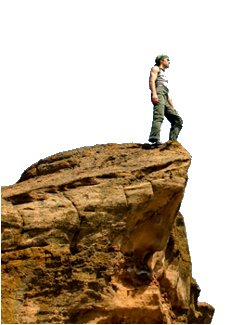
\includegraphics[width=4cm]{images/motivation}
\caption{Motivación.}
\end{figure}


\column{.5\textwidth}




\begin{block}{Tenemos...}

 \begin{itemize}[<+-| alert@+>]
        \item Conceptos clave: interoperabilidad, integración, soa y semántica.
        \item Tecnologías asociadas a estos conceptos.
        \item Tendencias en el desarrollo.
        \item y...¡un escenario de aplicación!.
\end{itemize}
\end{block}

\end{columns}

}


\frame{
  \frametitle{Contexto}

\begin{block}{E2000 Nuevas Tecnologías}

 \begin{itemize}[<+-| alert@+>]
        \item División de informática~\footnote{\url{http://www.e2000.es}} de la
asociación E2000 de mediadores de seguros.
        \item +500 asociados (clientes de negocio).
        \item Servicios de negocio: multitarificación, contratación,
declaración de siniestros, etc.
        \item Servicios técnicos de las aseguradores.
        \item Pasarela de comunicación con las aseguradoras SIA.
\end{itemize}
\end{block}


}


\frame{
  \frametitle{Contexto}

\begin{figure}[htb]
\centering
	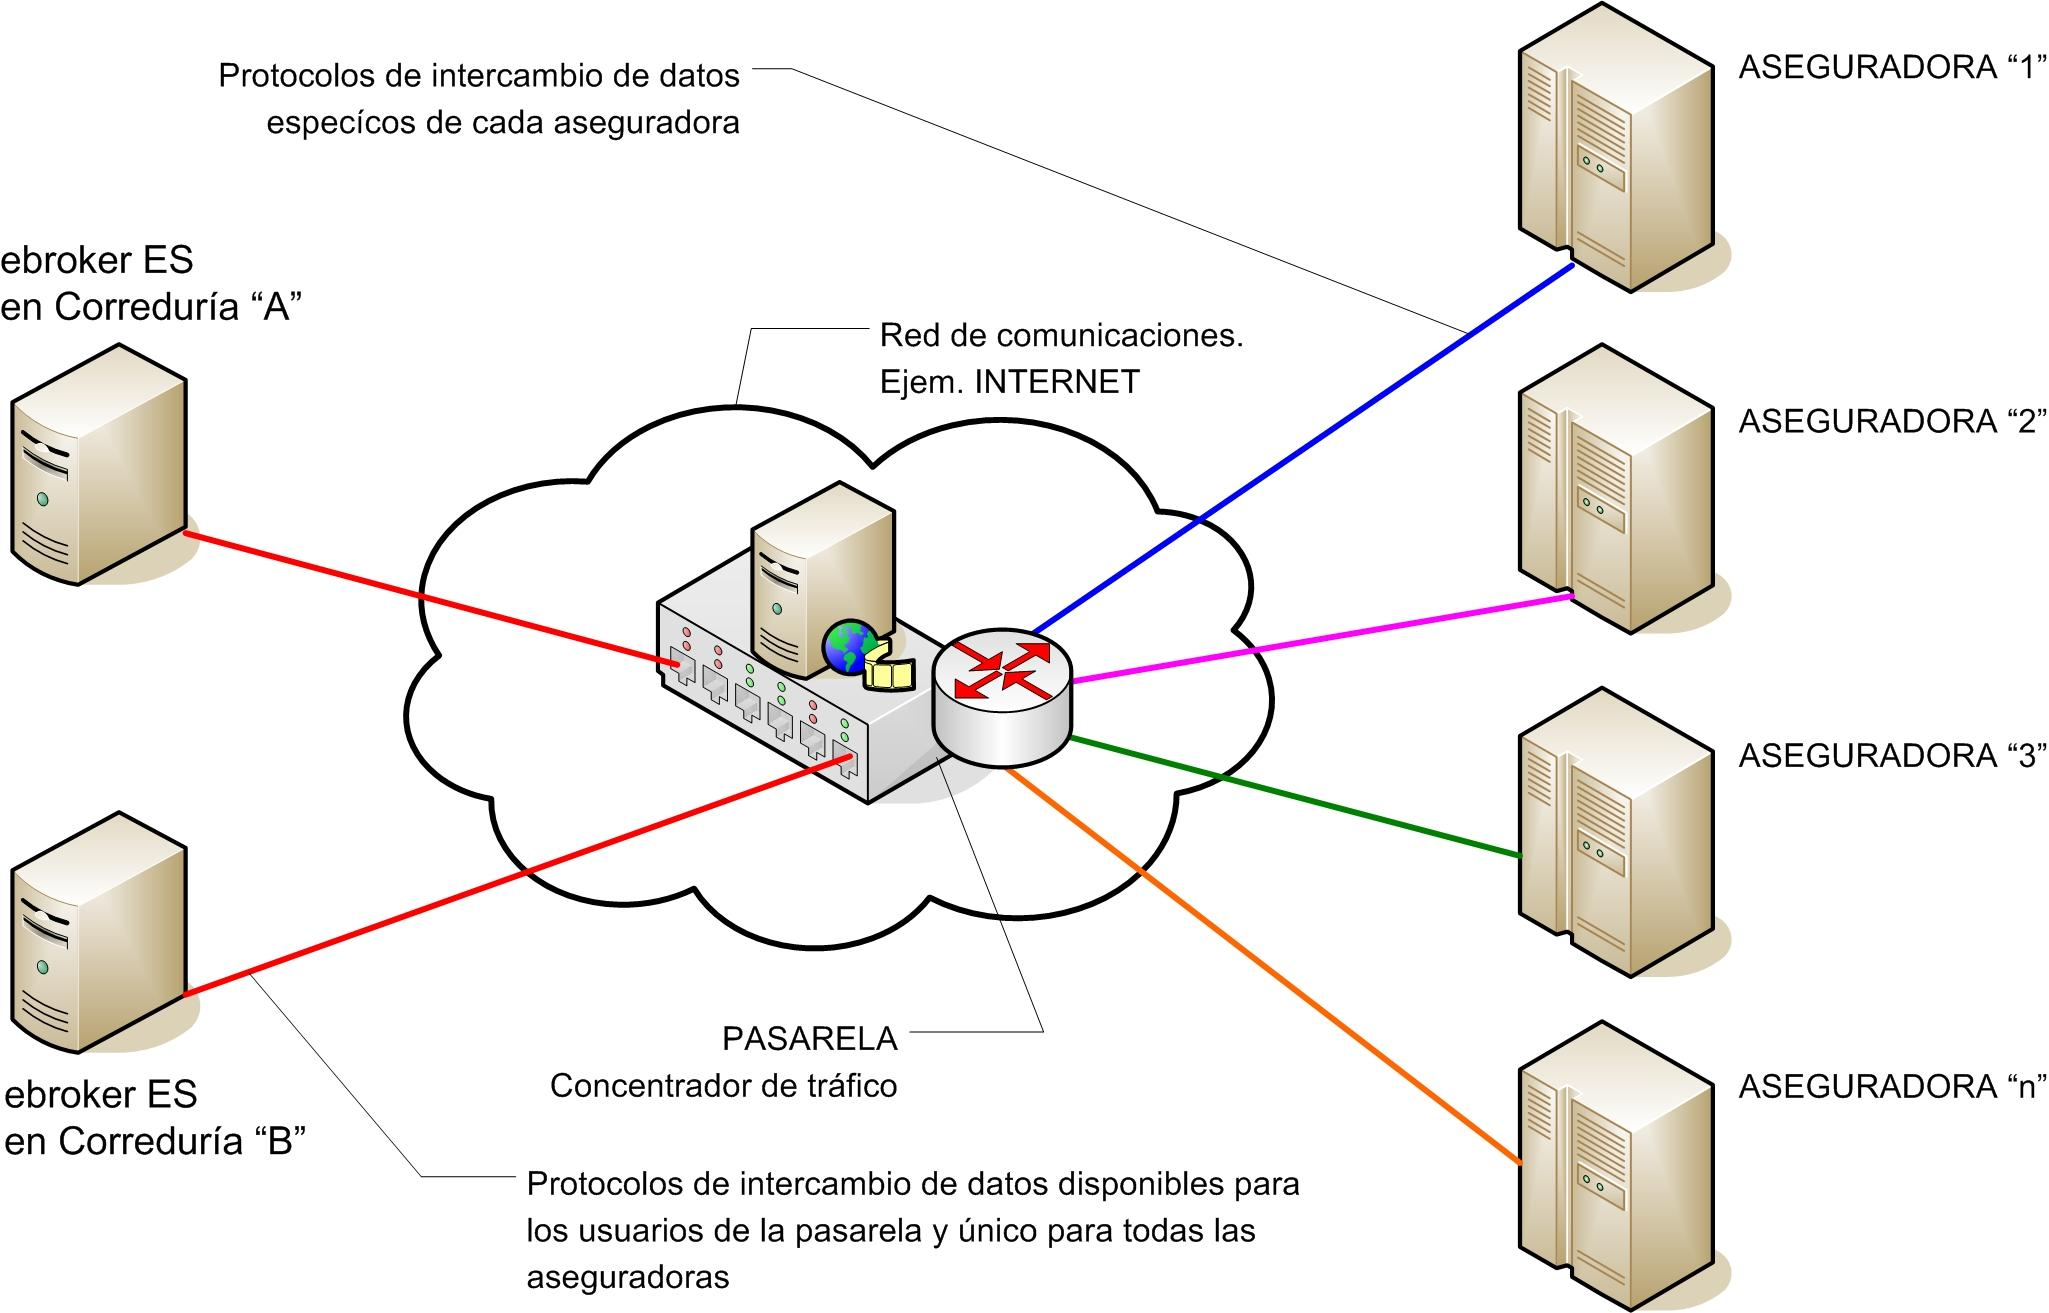
\includegraphics[width=8cm]{images/pasarela-sia}
\caption{Pasarela SIA de E2000.}
\end{figure}

}


\frame{
  \frametitle{Un poco de historia...}

Al principio pocas aseguradoras tenían servicios...

\begin{figure}[htb]
\centering
	
\includegraphics[width=4cm]{images/1-servicios}
\caption{Servicios en SIA (I).}
\end{figure}

}


\frame{
  \frametitle{...}

Las aseguradoras vieron el impacto de esta asociación y se fueron sumando...

\begin{figure}[htb]
\centering
	
\includegraphics[width=6cm]{images/2-servicios}
\caption{Servicios en SIA (II).}
\end{figure}

}


\frame{
  \frametitle{...}

Los asociados también eran más competitivos si había más aseguradoras...

\begin{figure}[htb]
\centering
  
\includegraphics[width=6cm]{images/3-servicios}
\caption{Servicios en SIA (III).}
\end{figure}

}



\frame{
  \frametitle{...pero...}

Creció y creció,...
\begin{figure}[htb]
\centering
	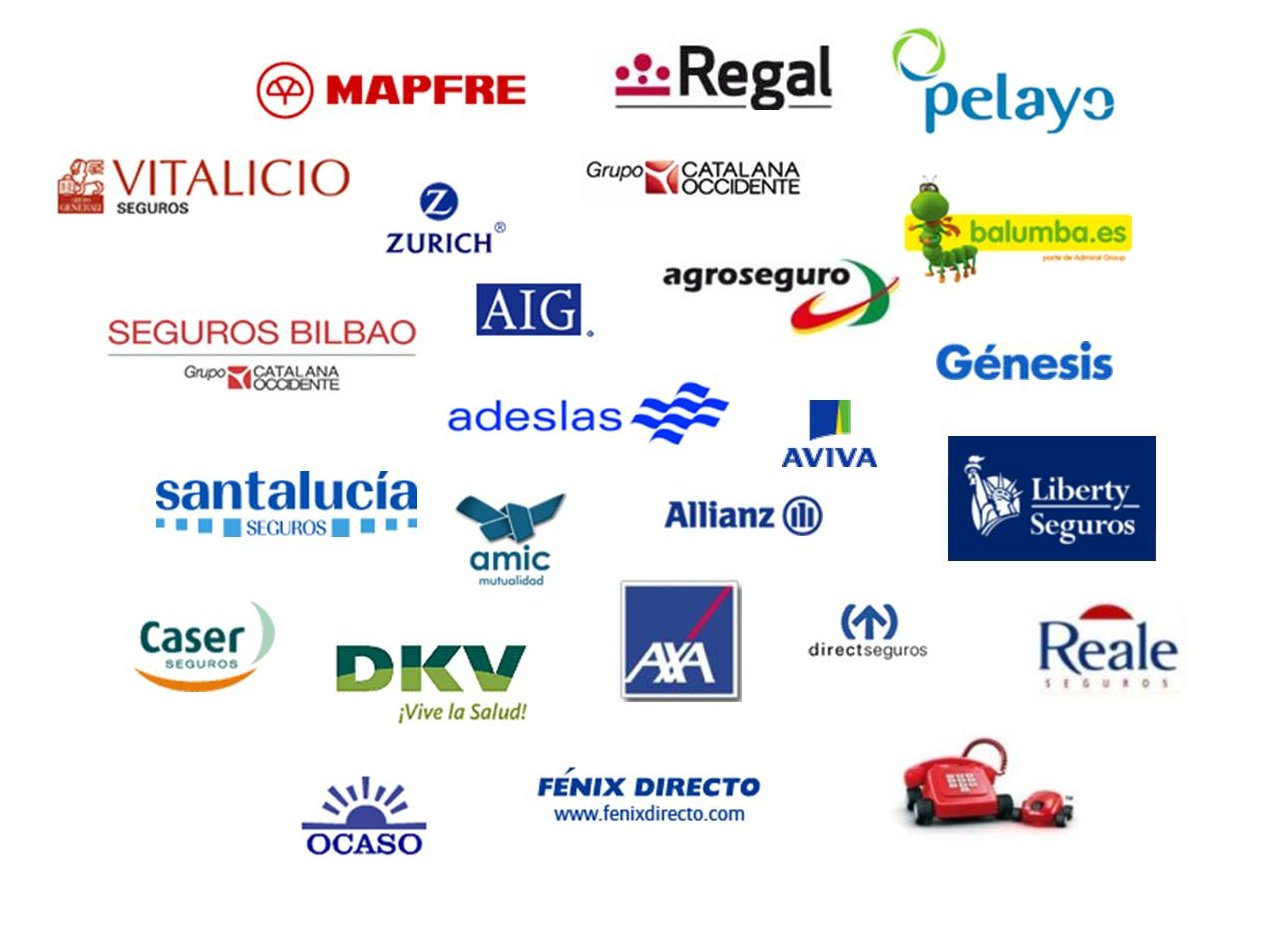
\includegraphics[width=6cm]{images/4-servicios}
\caption{Servicios en SIA (IV).}
\end{figure}

y aparecieron dificultades...

}

\frame{
  \frametitle{Dificultades}

\begin{figure}[htb]
\centering
	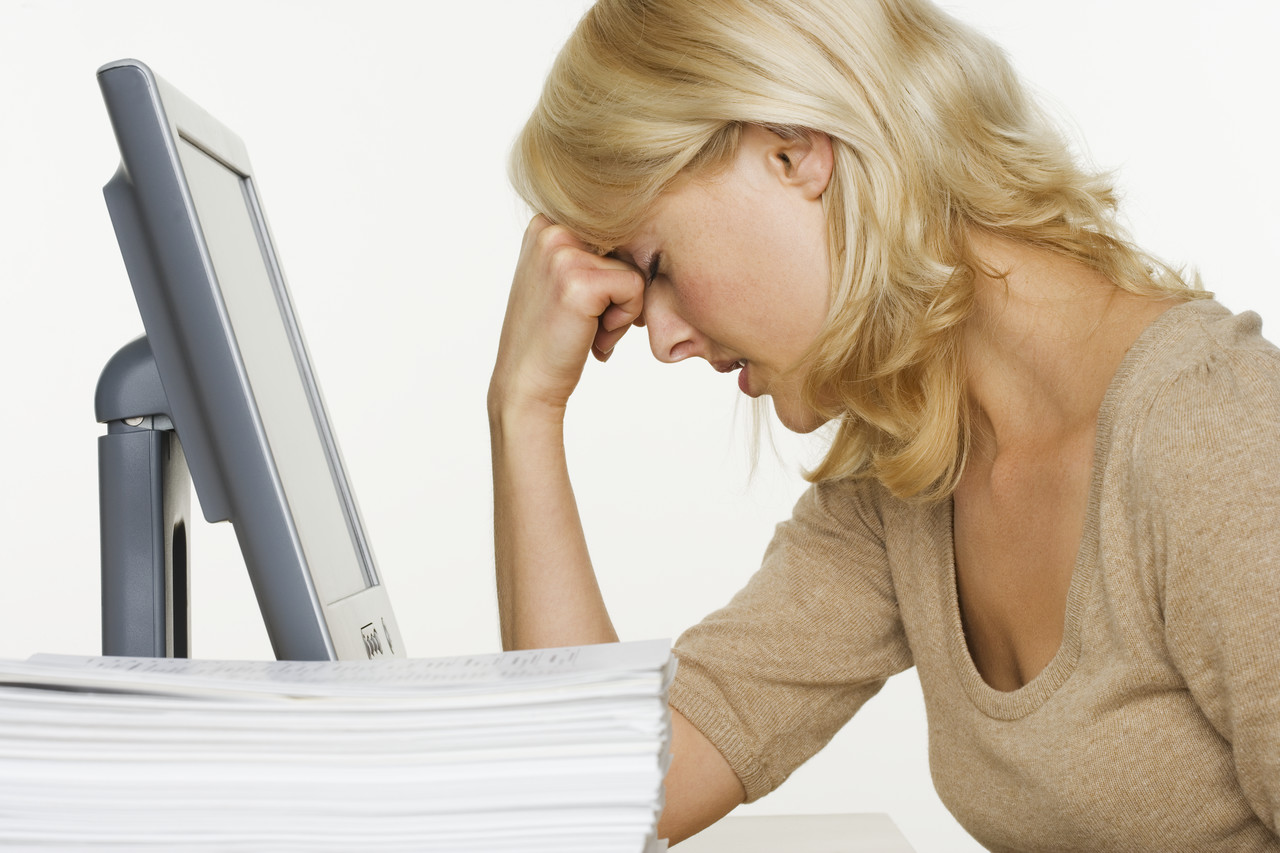
\includegraphics[width=6cm]{images/stress}
\caption{Primeras dificultades}
\end{figure}



}


\frame{
  \frametitle{Interoperabilidad}

Modelos de datos diferentes para la misma realidad.

\begin{columns}[c] % the "c" option specifies center vertical alignment
\column{.5\textwidth} % column designated by a command


\begin{figure}[htb]
\centering
	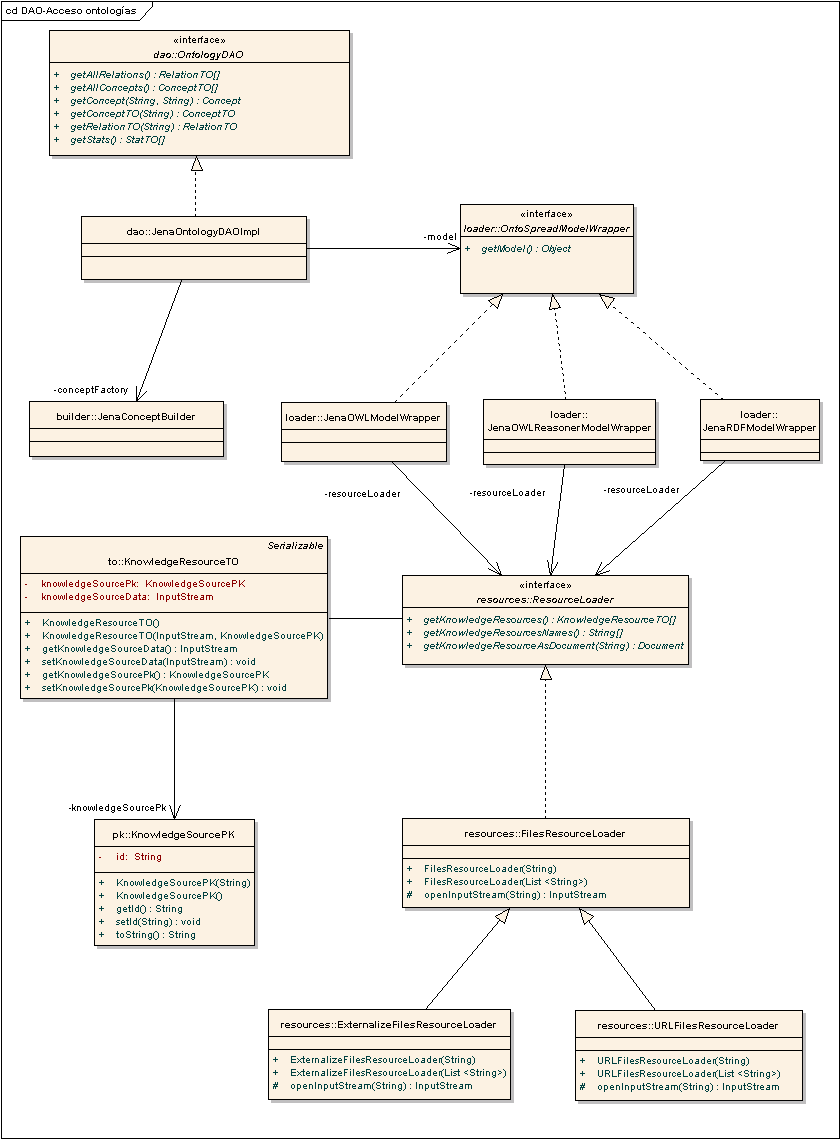
\includegraphics[width=4cm]{images/dao}
\caption{Estructurado.}

\end{figure}


\column{.5\textwidth}


\begin{figure}[htb]
\centering
	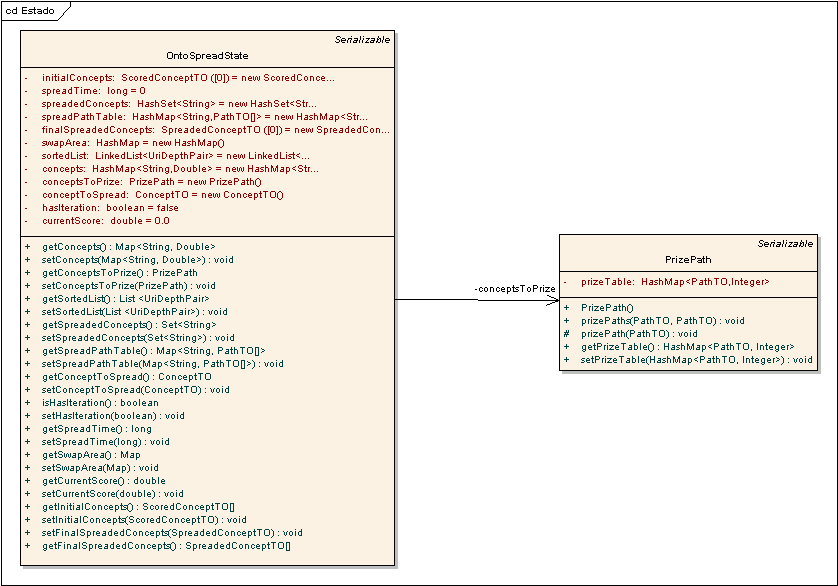
\includegraphics[width=4cm]{images/estado}
\caption{``Plano''.}

\end{figure}

\end{columns}





}

\frame{
  \frametitle{Integración}

Modelos de comunicación heterogéneos: protocolos, etc.

\begin{figure}[htb]
\centering
	\includegraphics[width=6cm]{images/integracion-servicios}
\caption{Integración}
\end{figure}

}


\frame{
  \frametitle{Resumiendo...}
\begin{alertblock}{Dificultades de SIA}

 \begin{itemize}[<+-| alert@+>]
        \item Presión de asociados y aseguradores por desplegar nuevos
servicios.
\item Muchas variantes en modelos de datos y comunicaciones para formalizar la
misma realidad.
\item La mayor parte del tiempo consumido en mantenimiento.
\item Descenso de la productividad.
\item Aumento de costes.
\end{itemize}
\end{alertblock}

}


\frame{
  \frametitle{...y...}


\begin{figure}[htb]
\centering
	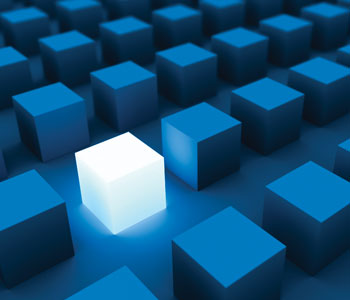
\includegraphics[width=6cm]{images/inovacion}
\caption{Idea.}
\end{figure}

}


\frame{
  \frametitle{...por qué no seguir un enfoque SOA+Semántica...}

\begin{exampleblock}{...consiguiendo:}

 \begin{itemize}[<+->]
\item Mejorar la interoperabilidad unificando los modelos de datos
utilizando estándares (RDF, OWL, etc.)
        \item Mejorar la integración de aplicaciones dentro de una
infraestructura (ESB).
\item Mantener un entorno para producción.
\item Dedicar tiempo para nuevos servicios.
\item Aumentar la productividad.
\item Disminuir costes.
\item Satisfacer a los asociados y a las aseguradoras.
\end{itemize}
\end{exampleblock}

}


\frame{
  \frametitle{Resultado}

  
\begin{columns}[c] % the "c" option specifies center vertical alignment
\column{.5\textwidth} % column designated by a command


\begin{figure}[htb]
\centering
	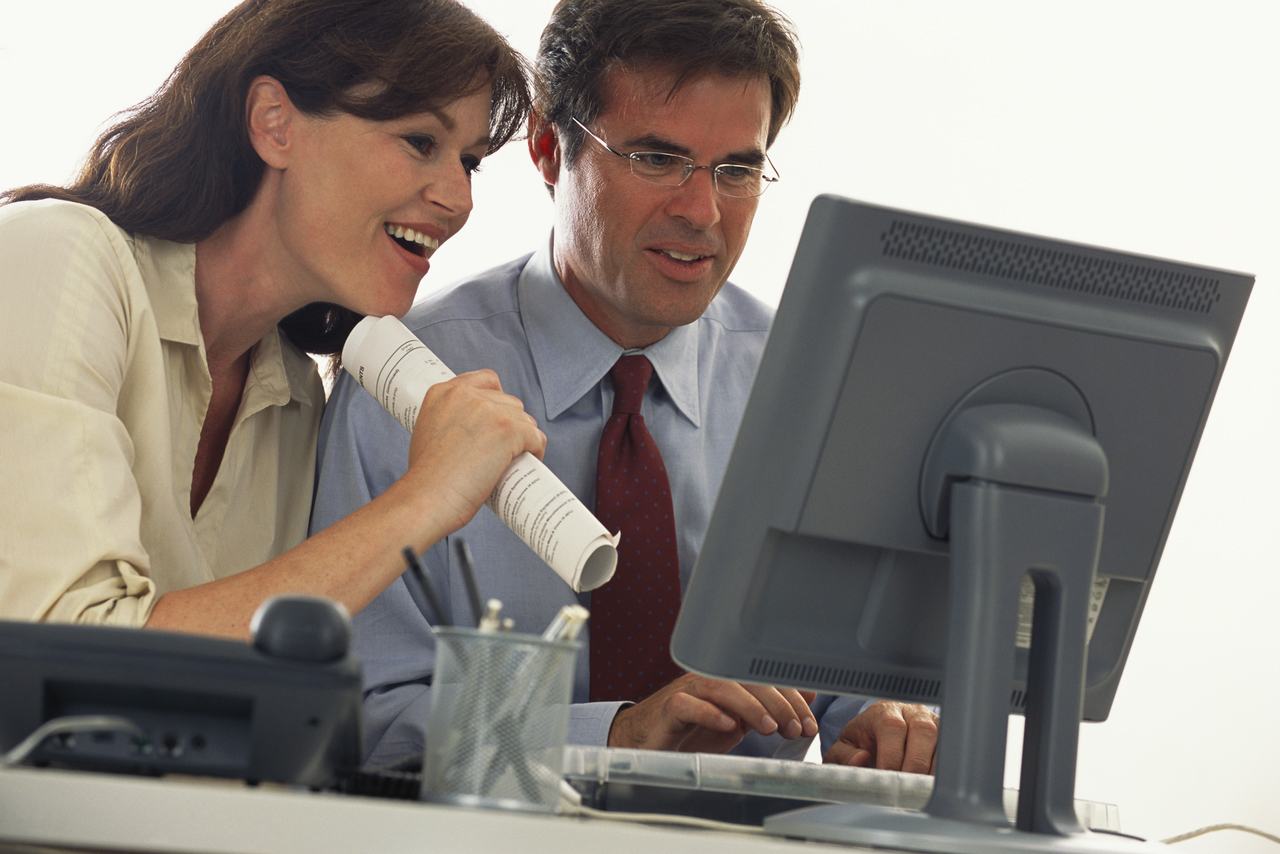
\includegraphics[width=4cm]{images/Programando-feliz}
\caption{Satisfacción de los Asociados y Desarrolladores.}
\end{figure}


\column{.5\textwidth}


\begin{figure}[htb]
\centering
	\includegraphics[width=4cm]{images/business-man}
\caption{Satisfacción de Ejecutivos.}
\end{figure}

\end{columns}

}


\frame{
  \frametitle{No es tan fácil...}

\begin{block}{Hay que investigar}
 \begin{itemize}[<+->]
\item Cómo podemos aplicar SOA manteniendo compatibilidad hacia atrás.
\item Cómo mejoramos la integración.
\item Cómo aplicamos semántica para mejorar la interoperabilidad.
\item Semántica+SOA. Qué propuestas hay: cubren las necesidades (producción,
etc.)
\end{itemize}
\end{block}

...pero de aquí nacen los objetivos.


}